\documentclass[compress,red]{beamer}
\usepackage{etex}
\mode<presentation>

\usetheme{Warsaw}
%\usetheme{Madrid}

\setbeamertemplate{navigation symbols}{}
\setbeamertemplate{headline}{}

\setbeameroption{show notes}
%\setbeameroption{hide notes}

%\hypersetup{pdfpagemode=FullScreen} % makes your presentation go automatically to full screen
%\useoutertheme[subsection=false]{smoothbars}
\useoutertheme{shadow}

% include packages
\usepackage{subfigure}
\usepackage{textcomp}
\usepackage{multicol}
\usepackage{amsmath}
\usepackage{epsfig}
\usepackage{graphicx}
\usepackage[all,knot]{xy}
\xyoption{arc}
\usepackage{url}
\usepackage{multimedia}
\usepackage{hyperref}
\usepackage{helvet}
\usepackage[english]{babel}
\usepackage[utf8]{inputenc}
\usepackage{multirow}
\usepackage{verbatim}
%\usepackage{geometry}
%\geometry{verbose,letterpaper}
%\usepackage{movie15}
%\usepackage{hyperref}
\usepackage{pgfpages}
\usepackage{setspace}


\graphicspath{{../pictures/}}

%\logo{}
\titlegraphic{\scalebox{4}{
    
\includegraphics[height=0.5cm]{ohwr_logo.eps}
  }
}


%\title{F*WATCH, making a watch differently!}
\title[{\makebox[.45\paperwidth]{F*WATCH\hfill%
       \insertframenumber/\inserttotalframenumber}}]{F*WATCH, making a watch differently!}


\author % (optional, use only with lots of authors)
{Federico Vaga, Matthieu Cattin}
% - Give the names in the same order as the appear in the paper.
% - Use the \inst{?} command only if the authors have different
%   affiliation.

%\institute%[Universities of Somewhere and Elsewhere] % (optional, but mostly needed)
%{
  %\inst{1}%
  %BE-CO Hardware and Timing section\\
  %CERN, Geneva, Switzerland
 %\and
 %\inst{2}%
 %Department of Theoretical Philosophy\\
 %University of Elsewhere
% }
% - Use the \inst command only if there are several affiliations.
% - Keep it simple, no one is interested in your street address.

\date %(optional, should be abbreviation of conference name)
{FOSDEM, Brussels, 31 January 2015}
% - Either use conference name or its abbreviation.
% - Not really informative to the audience, more for people (including
%   yourself) who are reading the slides online

%\subject{Theoretical Computer Science}
% This is only inserted into the PDF information catalog. Can be left
% out.


% If you have a file called "university-logo-filename.xxx", where xxx
% is a graphic format that can be processed by latex or pdflatex,
% resp., then you can add a logo as follows:

%\pgfdeclareimage[height=1cm]{ohr-logo}{ohr_logo.jpg}
%\logo{\pgfuseimage{ohr-logo}}


% Delete this, if you do not want the table of contents to pop up at
% the beginning of each subsection:
%\AtBeginSection[]
%{
%  \begin{frame}<beamer>{Outline}
%    \tableofcontents[currentsection]
%  \end{frame}
%}


% If you wish to uncover everything in a step-wise fashion, uncomment
% the following command:

%\beamerdefaultoverlayspecification{<+->}

\begin{document}

\begin{frame}
  \titlepage
  \note[item]{Federico: software engineer}
  \note[item]{Metthieu: electronic engineer}
  \note[item]{CERN BE-CO}.
  \note[item]{free time project}
\end{frame}

%\begin{frame}{Outline}
%  \tableofcontents
  % You might wish to add the option [pausesections]
%\end{frame}


% Structuring a talk is a difficult task and the following structure
% may not be suitable. Here are some rules that apply for this
% solution:

% - Exactly two or three sections (other than the summary).
% - At *most* three subsections per section.
% - Talk about 30s to 2min per frame. So there should be between about
%   15 and 30 frames, all told.

% - A conference audience is likely to know very little of what you
%   are going to talk about. So *simplify*!
% - In a 20min talk, getting the main ideas across is hard
%   enough. Leave out details, even if it means being less precise than
%   you think necessary.
% - If you omit details that are vital to the proof/implementation,
%   just say so once. Everybody will be happy with that.



%#####################################################################
%############ SECTION ################################################
\section{Introduction}

\subsection*{} % dummy subsection to display dots

%------------ FRAME --------------------------------------------------
\begin{frame}{What is it?}
  \begin{center}
    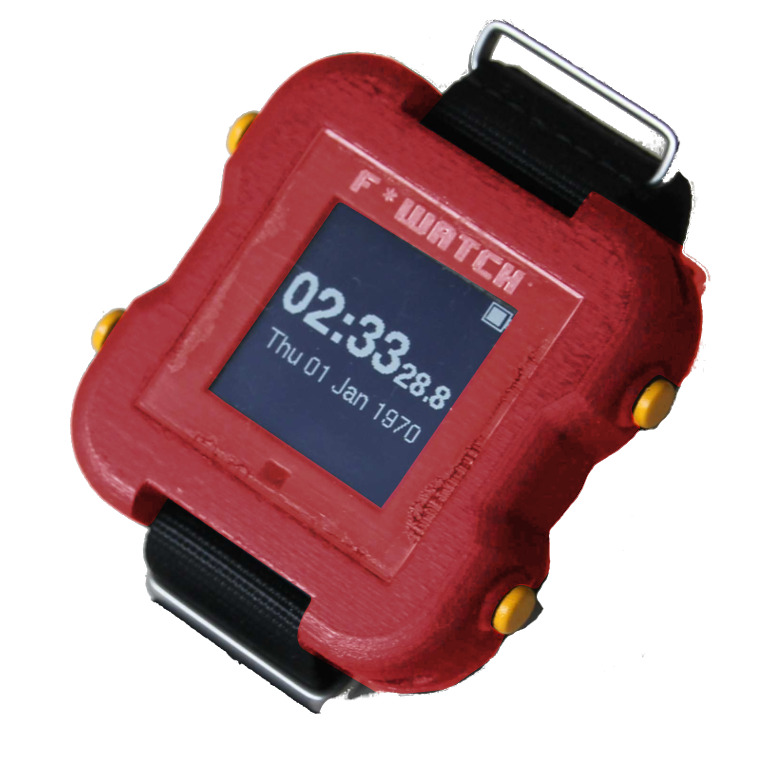
\includegraphics[height=7.5cm]{fwatch-full-side-red.eps}
  \end{center}
  \note[item]{This is a GPS watch}
  \note[item]{A lot of sensors}
  \note[item]{B/W screen}
  \note[item]{no touch screen --- buttons}
  \note[item]{other components --- not all}
  \note[item]{GPS module}
  \note[item]{it can run applications (smart watch)}
  \note[item]{Free product}
\end{frame}

%------------ FRAME --------------------------------------------------
\begin{frame}{Why a watch?}

  Retirement gift for a timing Hacker \\

  \textit{image: Julian face here?}
  
  \begin{enumerate}
    \item customization of the gift
    \item hackable gift
    \item free/open source
  \end{enumerate}

  \note[item]{Retirement timing hacker}
  \note[item]{currently, not free smart device}
  \note[item]{challange do it --- with free tools}

\end{frame}

%------------ FRAME --------------------------------------------------
\begin{frame}{Development organization}
  \begin{center}
    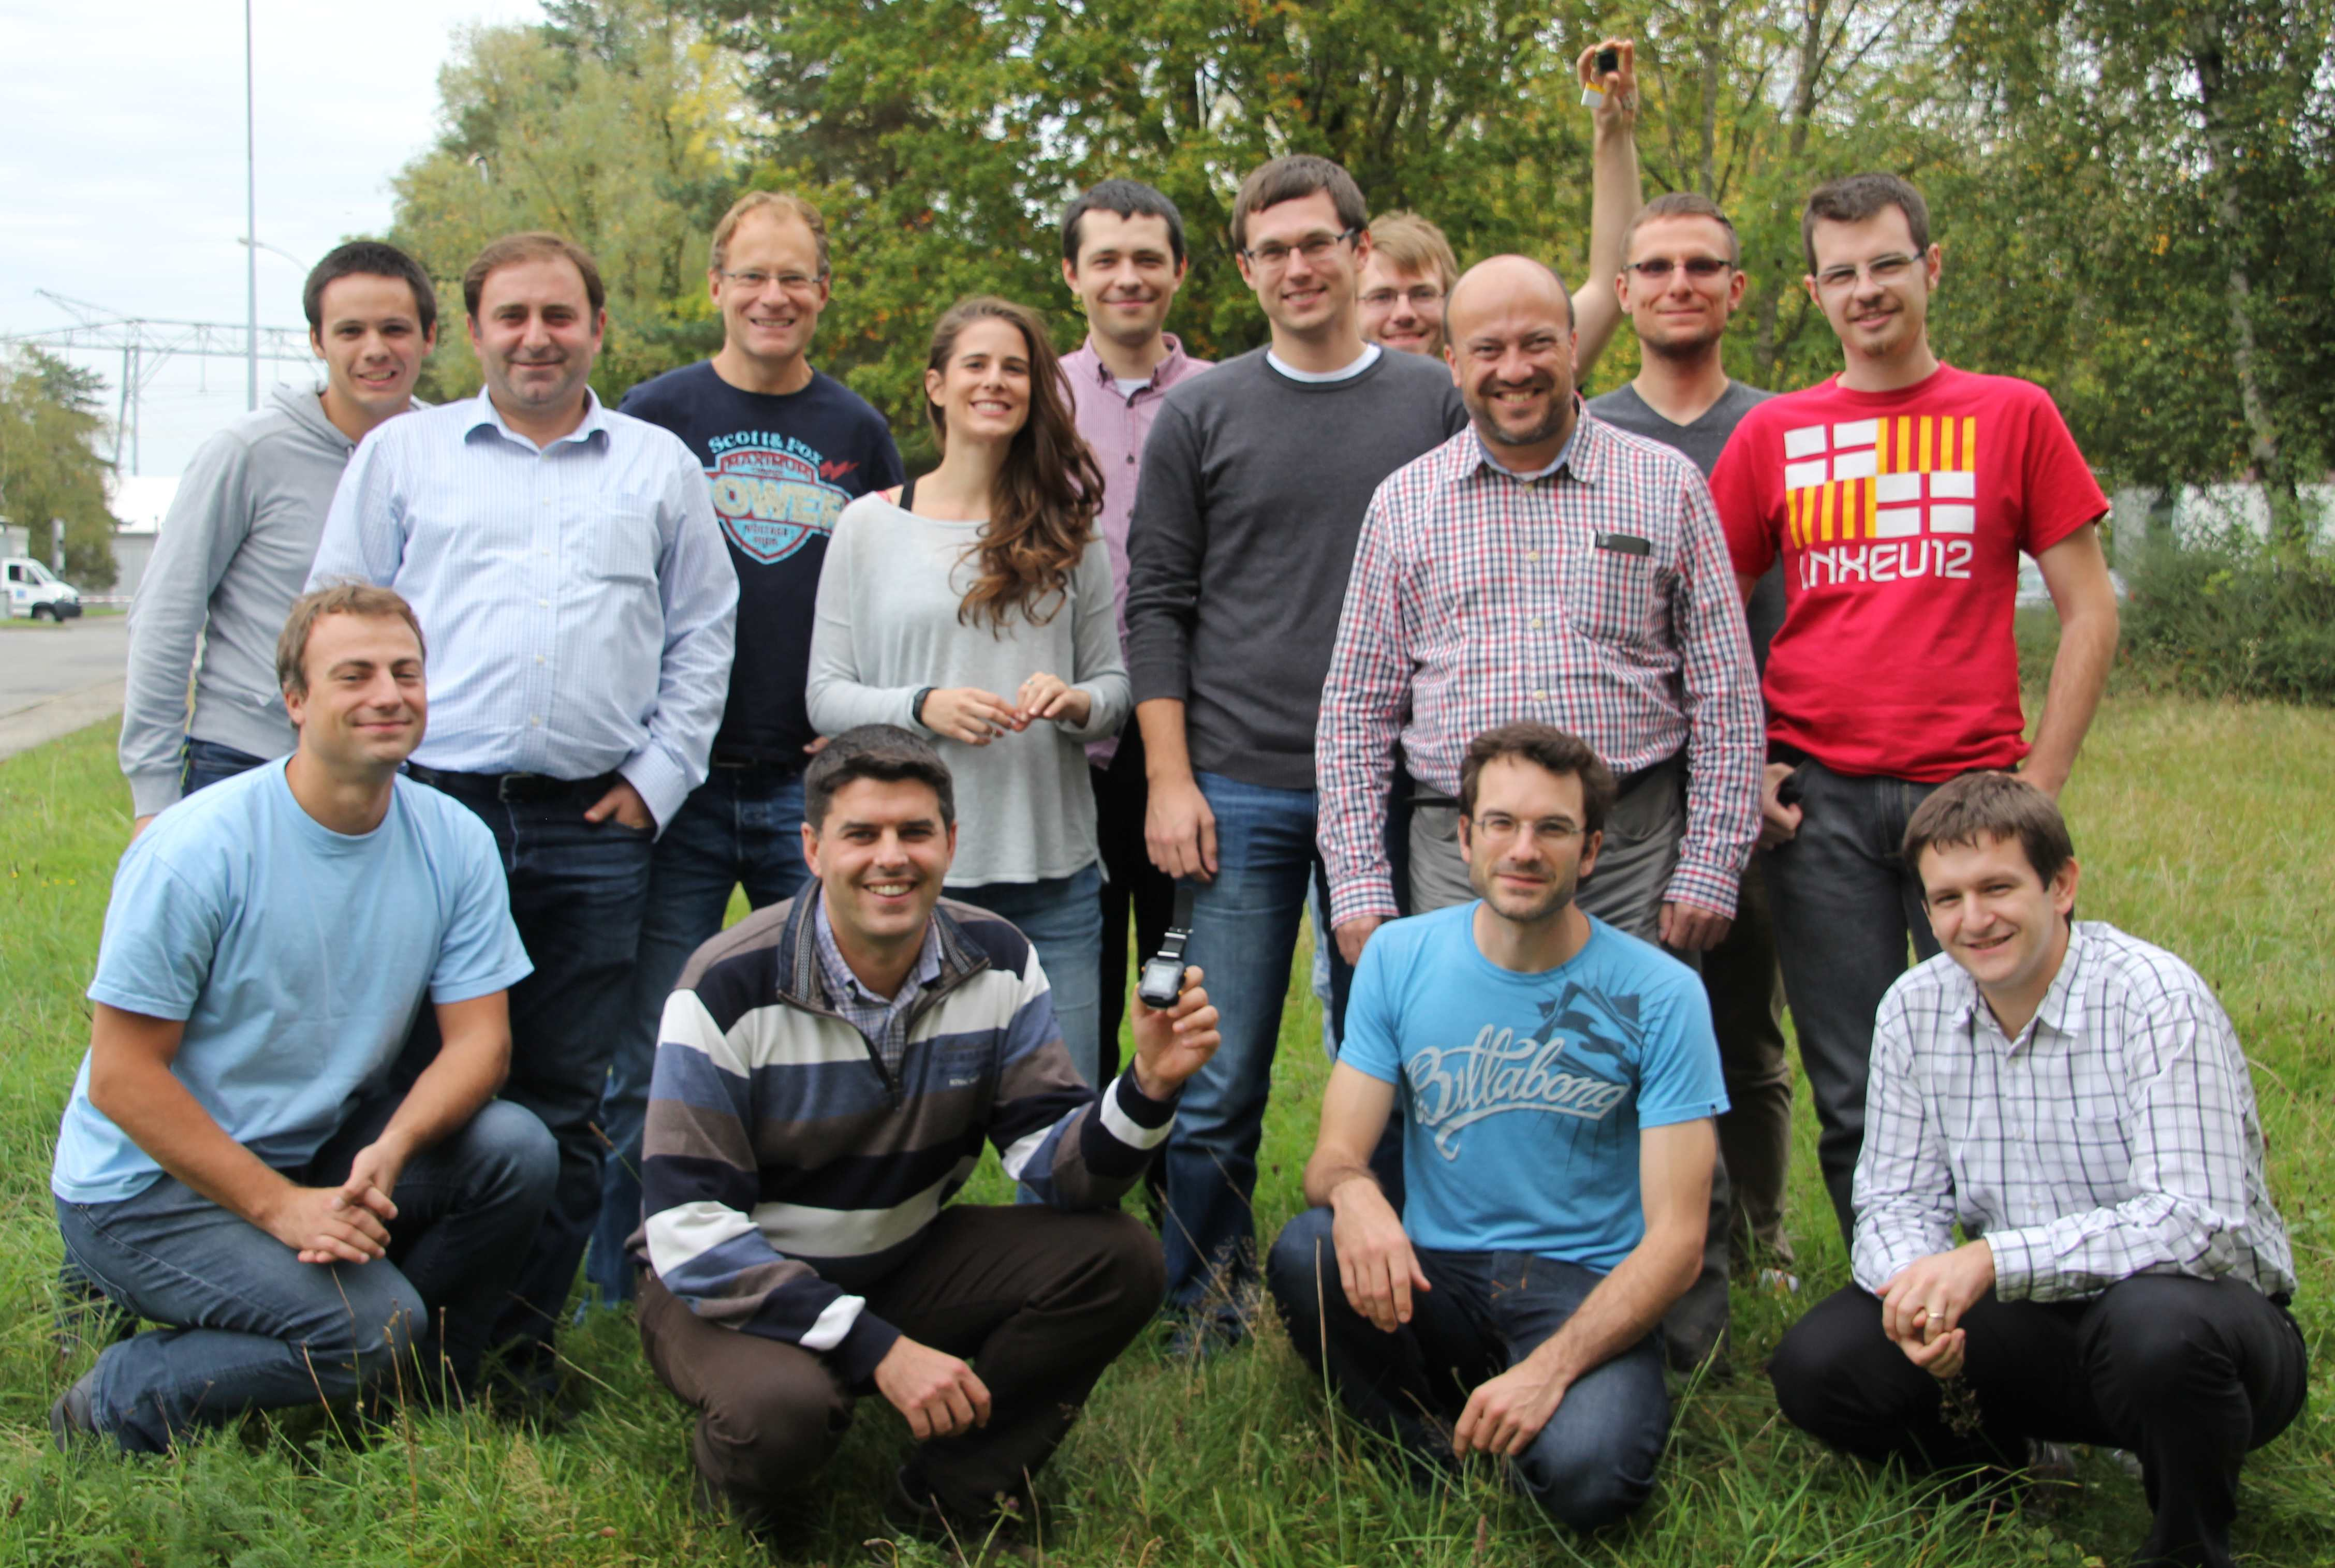
\includegraphics[height=7cm]{fwatch-team.eps}
  \end{center}

  \note[item]{people more or less involved}
  \note[item]{less than 5 months}
  \note[item]{after-work --- only free time}
  \note[item]{3 groups : mechanic, electronic, software}
  \note[item]{weekly meeting}
  \note[item]{introduce matthieu}
\end{frame}

%------------ FRAME --------------------------------------------------
%% \Large
%% \begin{frame}{Features}
%%   \begin{itemize}
%%     \item Low power MCU
%%     \item LCD display
%%     \item Sensors
%%     \item I/O interface
%%     \item GPS module
%%   \end{itemize}
%% \end{frame}


%#####################################################################
%############ SECTION ################################################
\section{The design}

%------------ FRAME --------------------------------------------------
\begin{frame}{Component selection}

  \begin{block}{Criteria}
    \begin{itemize}
    \item Low power consumption
    \item Available from main suppliers
    \item Small footprint
    \item ...
    \end{itemize}
  \end{block}

  \note[item]{}

\end{frame}

%------------ FRAME --------------------------------------------------
\begin{frame}{GPS module}

  \begin{block}{M10478-A1}
    \begin{itemize}
    \item Antenova
    \item 13 x 9.5 x 1.8mm
    \item Integrated antenna
    \end{itemize}
  \end{block}

  \begin{center}
    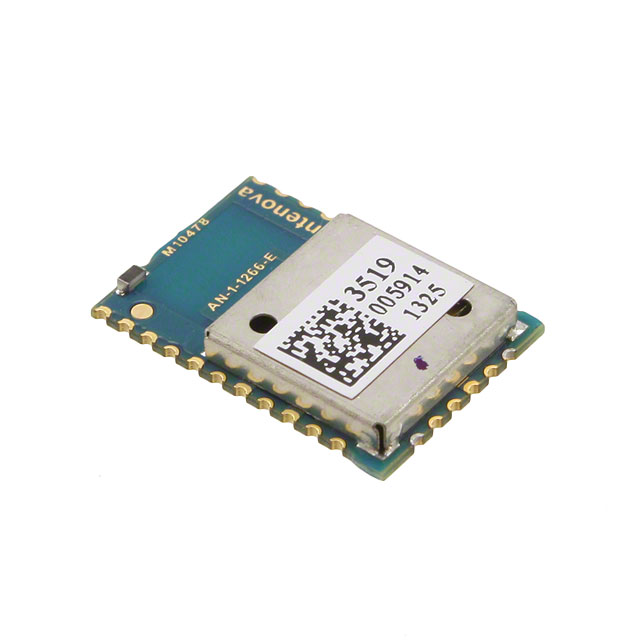
\includegraphics[height=5cm]{M10478-A1.eps}
  \end{center}

  \note[item]{}

\end{frame}

%------------ FRAME --------------------------------------------------
\begin{frame}{Altimeter module (pressure sensor)}

  \begin{block}{MS5806-02BA}
    \begin{itemize}
    \item Measurement Specialties
    \item 6.4 x 4 x 2.8mm
    \item Water resistant
    \end{itemize}
  \end{block}

  \begin{center}
    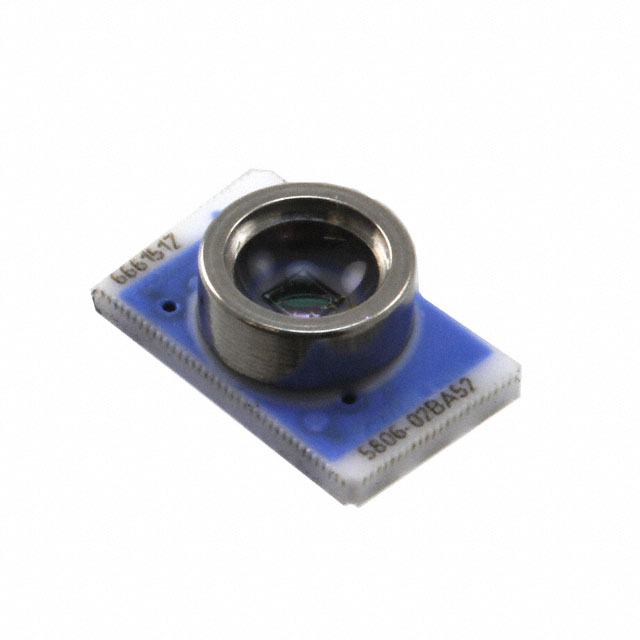
\includegraphics[height=4.5cm]{MS5806-02BA52-51.eps}
  \end{center}

  \note[item]{}

\end{frame}

%------------ FRAME --------------------------------------------------
\begin{frame}{Display}

  \begin{block}{Memory LCD}
    \begin{itemize}
    \item Sharp
    \item 128 x 128 pixels (1.28 inches)
    \item Ultra low current
    \end{itemize}
  \end{block}


  \begin{center}
    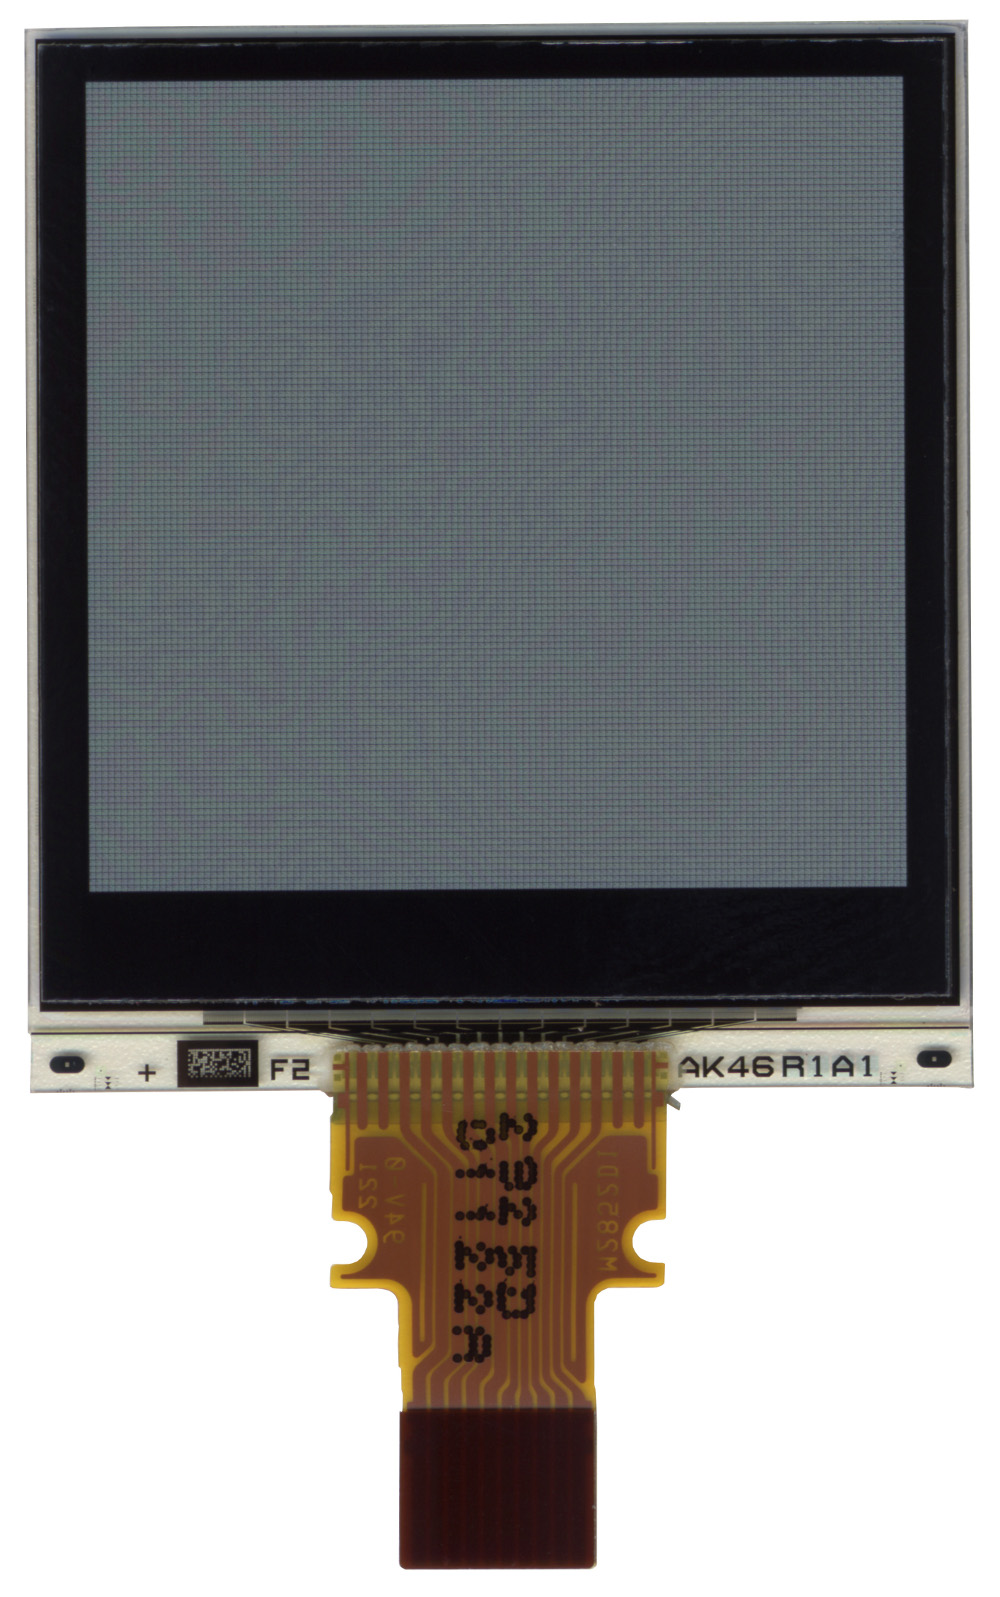
\includegraphics[height=4.5cm]{LCD.eps}
  \end{center}

  \note[item]{}

\end{frame}

%------------ FRAME --------------------------------------------------
\begin{frame}{Battery}

  \begin{block}{}
    \begin{itemize}
    \item Adafruit
    \item Li-ion 500mAh
    \item Lightweight, big capacity
    \end{itemize}
  \end{block}

  \begin{center}
    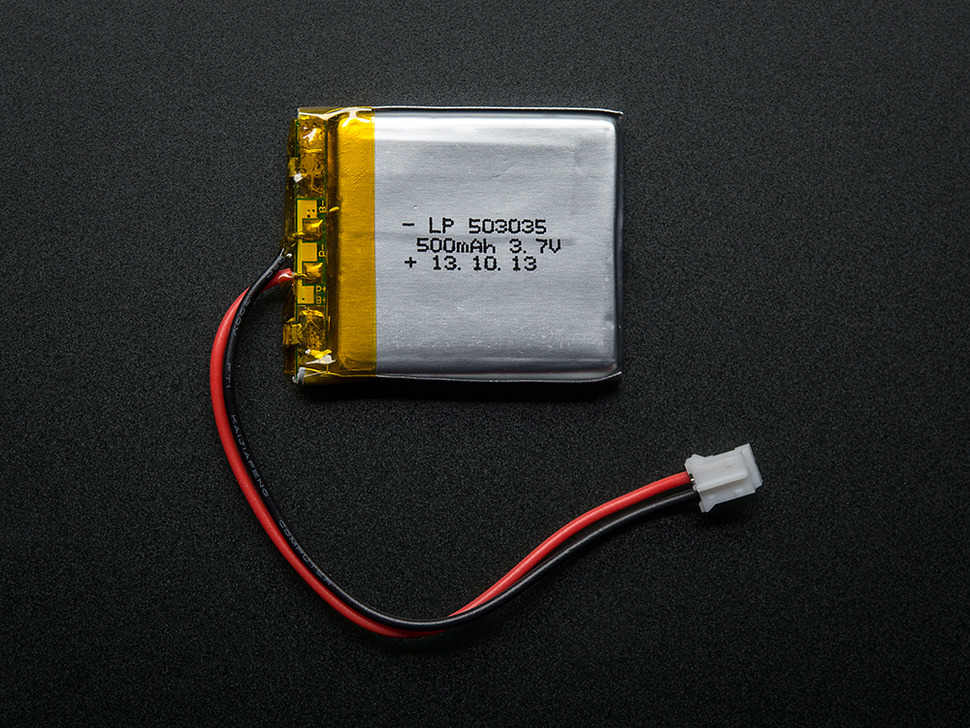
\includegraphics[height=5cm]{battery.eps}
  \end{center}

  \note{battery}
\end{frame}

%------------ FRAME --------------------------------------------------
\begin{frame}{Backlight}

  \begin{block}{A long story...}
    \begin{enumerate}
    \item LEDs + opaque plexiglass = fail
    \item Recycled smartphone backlight = works fine, but can't be sell as a kit
    \item Custom-made backlight = testing it now, promissing, cheap even in small quantity!
    \end{enumerate}
  \end{block}

  \begin{center}
    Backlight pictures here
    %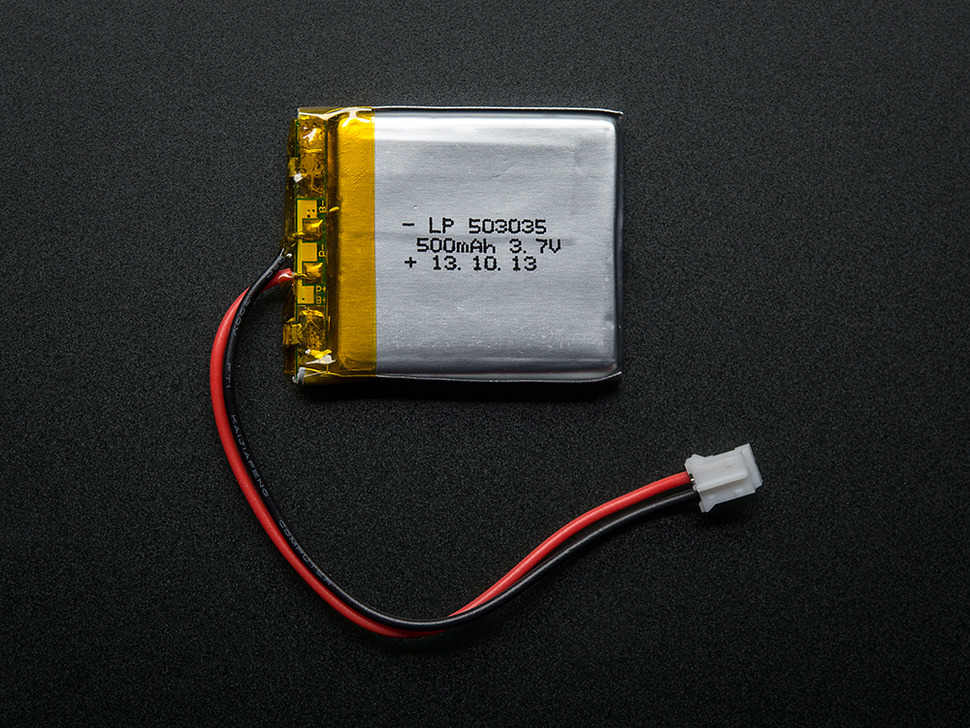
\includegraphics[height=5cm]{battery.eps}
  \end{center}

  \note[item]{}
\end{frame}

%------------ FRAME --------------------------------------------------
\begin{frame}{PCB design}

  \begin{block}{EDA tool choice}
    \begin{itemize}
    \item KiCad
    \item CERN is contributing
    \item Developer next door (help, bugfix, feedback)
    \item New features making routing easier
    \end{itemize}
  \end{block}

  \begin{block}{Interested in knowing more about KiCad developments?}
    \begin{itemize}
    \item Visit the EDA tools dev room tomorrow
    \end{itemize}
  \end{block}

  \begin{center}
    
\includegraphics[height=1cm]{kicad_logo.eps}
  \end{center}

  \note[item]{}
\end{frame}

%------------ FRAME --------------------------------------------------
\begin{frame}{PCB design}

  \begin{block}{Characteristics}
    \begin{itemize}
    \item 4 x 4 cm
    \item 4 layers
    \item Components on both sides
    \item Manufactered by Eurocircuits
    \end{itemize}
  \end{block}

  \begin{center}
    PCB top and bottom pictures here
    %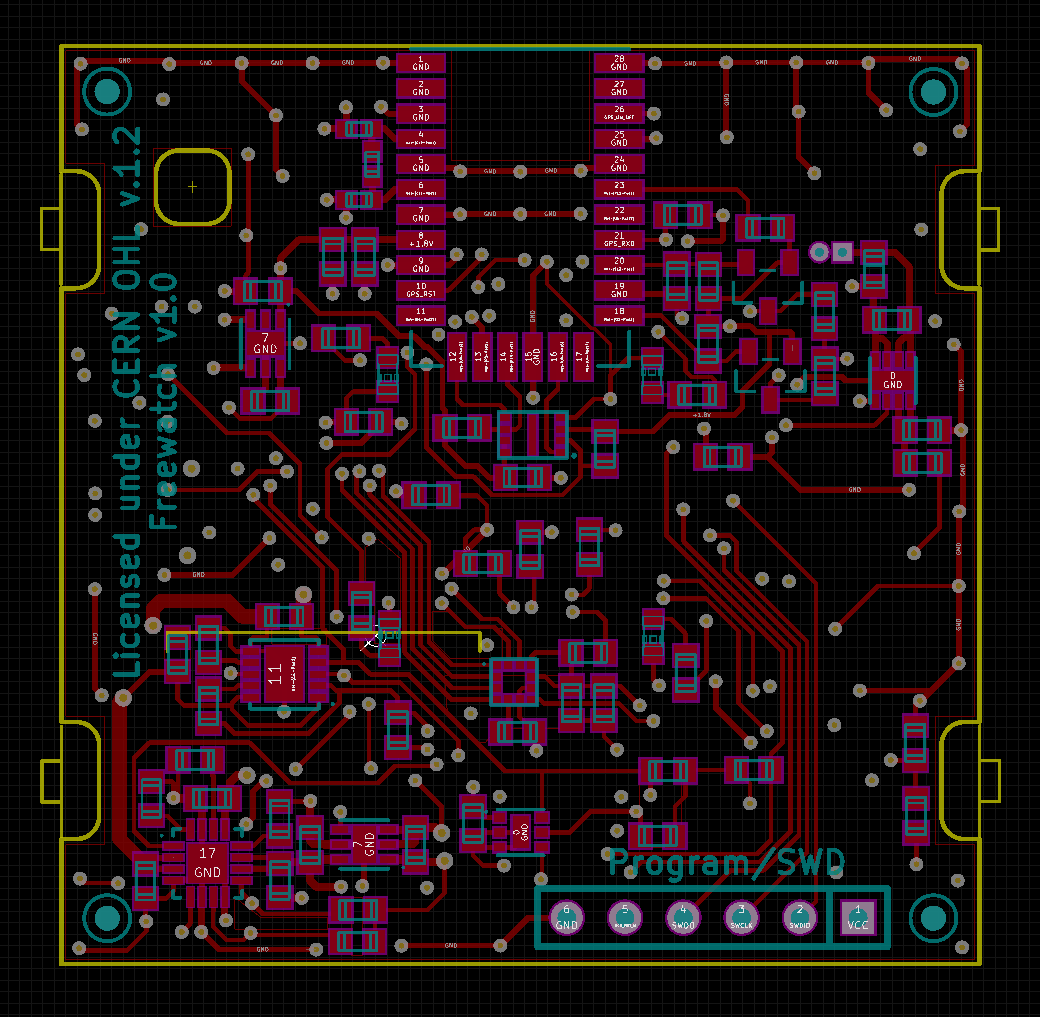
\includegraphics[height=1cm]{pcb_top.eps}~
    %\includegraphics[height=1cm]{pcb_bot.eps}
  \end{center}

  \note[item]{}
\end{frame}

%------------ FRAME --------------------------------------------------
\begin{frame}{PCB validation}

  \begin{block}{First prototype fully working, except two minor bugs}
    \begin{itemize}
    \item Error in a footprint
      \begin{itemize}
      \item Voltage regulator output wrongly set
      \end{itemize}
    \item MCU interrupt scheme
      \begin{itemize}
      \item No all MCU pins can be used as interrupt source
      \item Polling is draining the baterry quickly
      \end{itemize}
    \item Fixed with few cuts and wires!
    \end{itemize}
  \end{block}

  \begin{center}
    mounted pcb pictures here
    %\includegraphics[height=1cm]{pcb_assembly.eps}
  \end{center}

  \note[item]{}
\end{frame}

%------------ FRAME --------------------------------------------------
\begin{frame}{Mechanical design}

  \begin{block}{CAD tool selection}
    \begin{itemize}
    \item No mechanical designer in the team
    \item Evaluate existing free CAD tools (Freecad, ...)
    \item Docmentation, support
    \item Leanring curve, user-friendliness
    \end{itemize}
  \end{block}

  \begin{itemize}
  \item Decided to use \textbf{Freecad}
  \end{itemize}

  \begin{center}
    
\includegraphics[height=2cm]{freecad_logo.eps}
  \end{center}
  \note{Mechanical design}
\end{frame}

%------------ FRAME --------------------------------------------------
\begin{frame}{Mechanical design}

  \begin{block}{Challenges}
    \begin{itemize}
    \item Learn Freecad
    \item Buttons
    \item Water-resistance (dropped for proto)
    \item Size
    \item Wrist-strap
    \item 3D printing (new for us)
    \end{itemize}
  \end{block}

  \note[item]{Learn Freecad = show the making of video}
  \note[item]{Button = show detailed cut-view of button and explain quickly}
  \note[item]{Water-resistance = show, explain grove and rubber join idea}
  \note[item]{Size = keep it reasonably small to be wearable on the wrist}
  \note[item]{Wrist-strap = easy to get "nato" type wrist-strap, bought online}
  \note[item]{3D printing = didn't knew the domain, studied the main 3d printing services, }
  \note[item]{}

\end{frame}

%------------ FRAME --------------------------------------------------
\begin{frame}{3D model}

  \begin{center}
    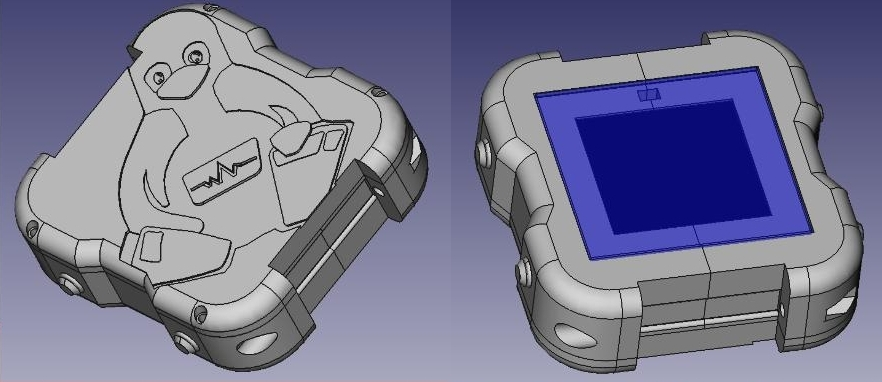
\includegraphics[height=4.8cm]{case-design-model.eps}
  \end{center}
  \note{3D model}
\end{frame}

%------------ FRAME --------------------------------------------------
\begin{frame}{First 3D print}

  \begin{itemize}
  \item Platic material (powder-based)
  \end{itemize}

  \begin{center}
    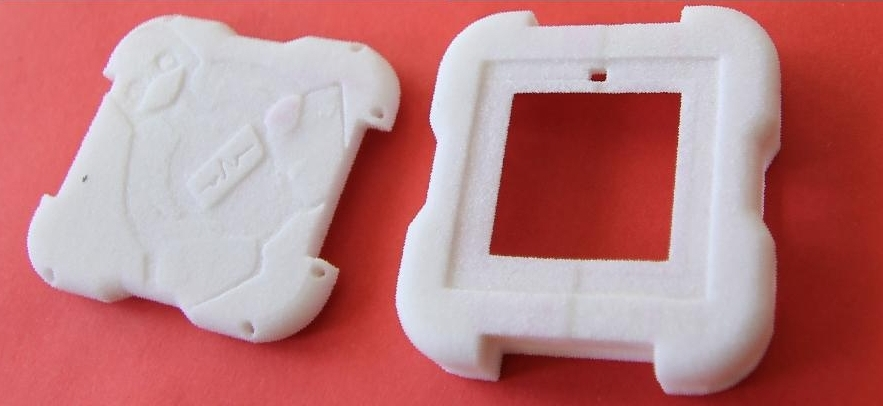
\includegraphics[height=5cm]{case-design-print-v2.eps}
  \end{center}
  \note{3D Model}
\end{frame}

%------------ FRAME --------------------------------------------------
\begin{frame}{Second 3D print}

  \begin{itemize}
  \item Resin material (liquid-based)
  \end{itemize}

  \begin{center}
    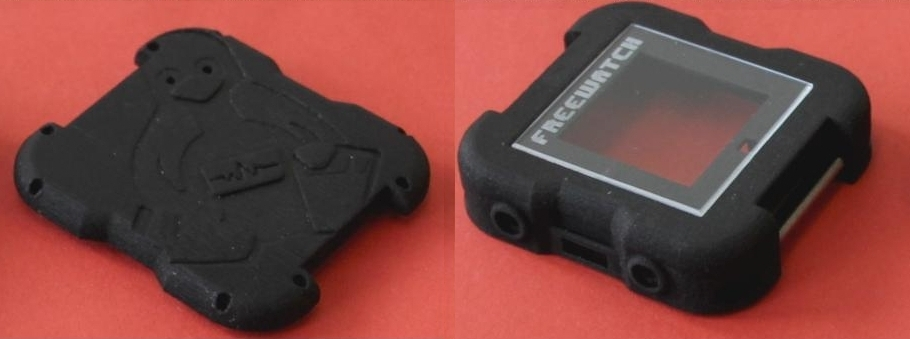
\includegraphics[height=4.1cm]{case-design-print-v3.eps}
  \end{center}
  \note{3D Model}
\end{frame}


%------------ FRAME --------------------------------------------------
\begin{frame}{Third 3D print}

  \begin{itemize}
  \item Resin material
  \item Improved case parts fastening
  \end{itemize}

  \begin{center}
    Picture of the new fastening method + transparent 3d view
    %\includegraphics[height=4.1cm]{case-design-print-v4.eps}
  \end{center}

\end{frame}



%#####################################################################
%############ SECTION ################################################
\section{Building a watch}

\subsection*{} % dummy subsection to display dots

%------------ FRAME --------------------------------------------------
\begin{frame}{Building the watch}

  \begin{block}{Components procurement}
    \begin{itemize}
    \item Buy electronics components
    \item Download PCB gerber file and order circuit
    \item Download 3D model and order from a 3D service
    \item Buy or build a programmer
    \end{itemize}
  \end{block}

  \note[item]{I want to build this watch, what should I do?}

\end{frame}

%------------ FRAME --------------------------------------------------
\begin{frame}{Building the watch}

  \begin{block}{Tools and techniques}
    \begin{itemize}
    \item Soldering QFN/BGA (stencil, paste)
    \item Hot-air station or oven
    \item Programmer to flash the booloader
    \item Optional: Milling maching (plexiglass)
    \end{itemize}
  \end{block}

  \note[item]{Or split in separte frames with a nice picture for each point??}
\end{frame}

%------------ FRAME --------------------------------------------------
\begin{frame}{Building the watch}

  \begin{block}{PCB assembly}
    \begin{itemize}
    \item Stencils (ordered with PCB)
    \item Leaded soldering paste (easier to handle than lead-free)
    \item Components placed by hand (script to generate placement pdf)
    \item Soldered with hot-air station (quite tricky!)
    \end{itemize}
  \end{block}

  \begin{center}
    %\includegraphics[height=1cm]{pcb_assembly.eps}
    %\includegraphics[height=1cm]{placement_pdf.eps}
  \end{center}

  \note[item]{}
\end{frame}

%------------ FRAME --------------------------------------------------
\begin{frame}{Building the watch}

  \begin{block}{Software}
    \begin{itemize}
    \item Download sources from the GIT repo
    \item Find your way through the sources (not nicely bundled, yet)
    \item Compile booloader and flash it (using a programmer)
    \item Compile application software and flash it (using the bootloader)
    \item Modify, re-flash, etc...
    \end{itemize}
  \end{block}

  \note[item]{}

\end{frame}

%------------ FRAME --------------------------------------------------
\begin{frame}{How much does it costs?}

  \begin{block}{Estimated cost for small series (without shipping)}

  \begin{table}[h]
    \begin{tabular}{l|r|r|r|l}
      \cline{2-4}
      & \multicolumn{3}{c|}{Number of watches}                                     &  \\ \cline{2-4}
      & \multicolumn{1}{c|}{1} & \multicolumn{1}{c|}{10} & \multicolumn{1}{c|}{50} &  \\ \cline{1-4}
      \multicolumn{1}{|l|}{Pcb + components}         & 166 \texteuro                & 87 \texteuro                  & 73 \texteuro                  &  \\ \cline{1-4}
      \multicolumn{1}{|l|}{Pcb assembly}             & -                      & 104 \texteuro                 & 59 \texteuro                  &  \\ \cline{1-4}
      \multicolumn{1}{|l|}{Case + buttons + screws}  & 67 \texteuro                 & 65 \texteuro                  & 60 \texteuro                  &  \\ \cline{1-4}
      \multicolumn{1}{|l|}{\textbf{TOTAL per watch}} & \textbf{233 \texteuro}       & \textbf{256 \texteuro}        & \textbf{193 \texteuro}        &  \\ \cline{1-4}
      \multicolumn{1}{|l|}{\textbf{TOTAL}}           & \textbf{233 \texteuro}       & \textbf{2'558 \texteuro}      & \textbf{9'630 \texteuro}      &  \\ \cline{1-4}
    \end{tabular}
  \end{table}

  \end{block}


  \note[item]{}
\end{frame}


%#####################################################################
%############ SECTION ################################################
\section{What's next?}

\subsection*{} % dummy subsection to display dots

%------------ FRAME --------------------------------------------------
\begin{frame}{What's next?}

  \begin{block}{Improvements}
    \begin{itemize}
    \item Bluetooth LE
    \item Water-resistance
    \item LCD backlight
    \item Reduce PCB/housing size
    \item 
    \end{itemize}
  \end{block}

  \begin{block}{Software}
    \begin{itemize}
    \item Firmware loader
    \item Data transfer (to/from SD card)
    \item Emulator
    \item Application "ecosystem"
      \begin{itemize}
      \item GPS route following
      \item Atmosheric pressure history
      \item Altitude based on atmospheric pressure
      \item ...
      \end{itemize}
    \end{itemize}
  \end{block}

  \note[item]{}

\end{frame}

%------------ FRAME --------------------------------------------------
\begin{frame}{What's next?}

  \begin{block}{Build a community}
    \begin{itemize}
    \item 
    \item 
    \end{itemize}
  \end{block}
  \note[item]{}

\end{frame}

%------------ FRAME --------------------------------------------------
\begin{frame}{What's next?}

  \begin{block}{Make a kit}
    \begin{itemize}
    \item Pre-assembled PCB option
    \item Customisable strap/housing color
    \item Alternative housing
    \item Sold by a company?
    \end{itemize}
  \end{block}

  \note[item]{}

\end{frame}

%#####################################################################
%############ SECTION ################################################
\section{Software}

\begin{frame}{MCU SDK}
  \Large
  \begin{center}
    Mainly open source software \\
    \vskip 1cm
    A lot of integration examples \\
    \vskip 1cm
    Well documented \\
  \end{center}

  \note{Say few things about the SDK}
\end{frame}

%------------ FRAME --------------------------------------------------

\begin{frame}{Bootloader}
  \Large
  \begin{center}
    free bootloader provided by SiliconLab \\
    \vskip 1cm
    support for IAR, Keil uVision \\
    \vskip 1cm
    migrate to gcc toolchain \\
    \vskip 1cm
    (don't use gcc optimization!)
  \end{center}

  \note{Few thing about the bootloader}
\end{frame}

%------------ FRAME --------------------------------------------------

\begin{frame}{Operating System}
 \large
 \begin{center}
  \begin{tabular}{lcccc}
    & FreeRTOS & uC/OS-III & RTX & TNKernel \\[2.5mm]
    \hline
    \\[1mm]
   License & Mod. GPL & restrictive & BSD & BSD \\[5mm]
   EFM32   & yes      & yes         & yes & no  \\[5mm]
   USB     & no       & yes         & no  & yes \\[5mm]
   FAT     & yes      & yes         & no  & yes \\
  \end{tabular}
 \end{center}

 \note[item]{License main thing}
 \note[item]{uC nice but closed}
 \note[item]{FreeRTOS --- Keil RTX}
\end{frame}

%------------ FRAME --------------------------------------------------

\begin{frame}{Operating System}
  \Large
  \begin{columns}[T] % align columns
    \begin{column}{.48\textwidth}
      FreeRTOS
      \vskip 1cm
      \begin{itemize}
      \item nice documentation
        \vskip 1cm
      \item big community
        \vskip 1cm
      \item a lot of examples
      \end{itemize}
    \end{column}
    \hfill%
    \begin{column}{.48\textwidth}
      Keil RTX
      \vskip 1cm
      \begin{itemize}
      \item nice documentation
        \vskip 1cm
      \item community?
        \vskip 1cm
      \item few examples
      \end{itemize}
    \end{column}%
  \end{columns}

  \note{The main criterium here was the level of knowledge sharing
    around the projects}
\end{frame}

%------------ FRAME --------------------------------------------------

\begin{frame}{Applications}
  \begin{center}
    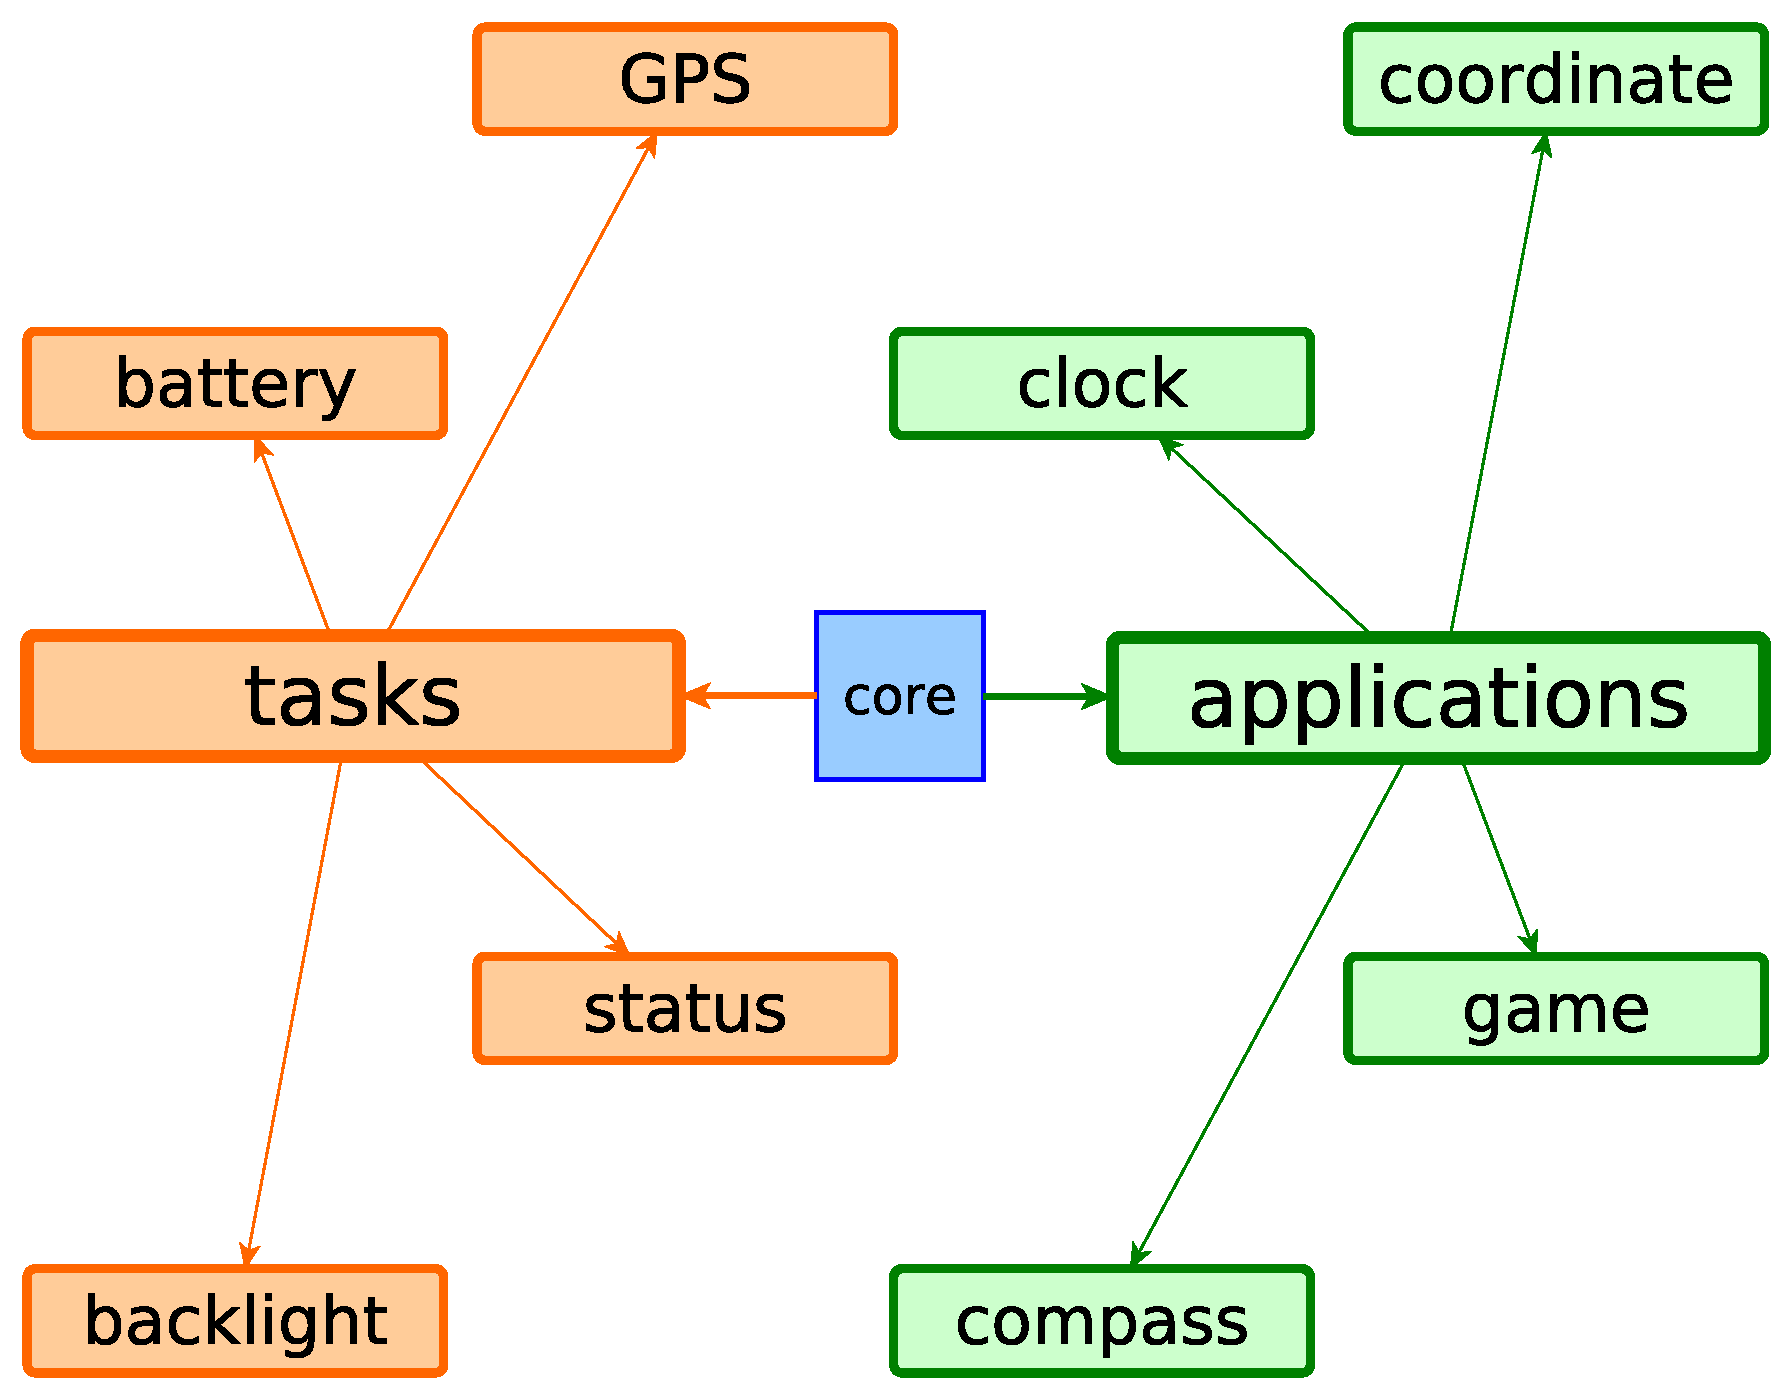
\includegraphics[height=7cm]{sw-app.eps}
  \end{center}

  \note{DO NOT SAY TOO MUCH, THERE WILL BE THE VIDEO LATER}
  \note[item]{task: say basically what they do}
  \note[item]{apps: say basically what they do}
\end{frame}

%------------ FRAME --------------------------------------------------

\begin{frame}
  \begin{center}
    \begin{figure}[h!]
      \centering
%  \movie[height=5cm, width = 5cm, autostart, once, showcontrols=true,
%borderwidth=1pt, poster]{Applications Demonstration}{bird.avi}
    \end{figure}
  \end{center}
  \note{just comment the video}
\end{frame}

%------------ FRAME --------------------------------------------------

\begin{frame}{Documentation}
  \Large
  \begin{center}
      www.ohwr.org/projects/f-watch/wiki
  \end{center}
  \vskip 1cm
  \begin{itemize}
  \item how to configure your machine
    \vskip 7mm
  \item how to write applications
    \vskip 7mm
  \item details about the project
  \end{itemize}

  \note{Few words about the project documentation}
\end{frame}

%#####################################################################
%############ SECTION ################################################
\section{Conclusions}

\begin{frame}{Development Summary}
  \Large
  \begin{columns}[T] % align columns
    \begin{column}{.55\textwidth}
      \begin{itemize}
      \item free PCB design
        \vskip 8mm
      \item free mechanic design
        \vskip 8mm
      \item free software
        \vskip 8mm
       \item free tools
      \end{itemize}
        \note[item]{just read list}
        \note[item]{Free Tools --- This is madness! --- Madness? This
          is Free Development!}
    \end{column}
    \hfill%
    \pause
    \begin{column}{.43\textwidth}
      \vskip 18mm
      \begin{center}
        \textbf{free} development \\
        for\\
        \textbf{free} products
      \end{center}
        \note[item]{A lot of good free tools for sw devel}
        \note[item]{free tools often crappy}
        \note[item]{fortunatelly today some of them are mature and
          competitive}
    \end{column}%
  \end{columns}
\end{frame}

%------------ FRAME --------------------------------------------------

\begin{frame}{Free Development Need Free Tools}
  \begin{center}
    \alt<2> {
      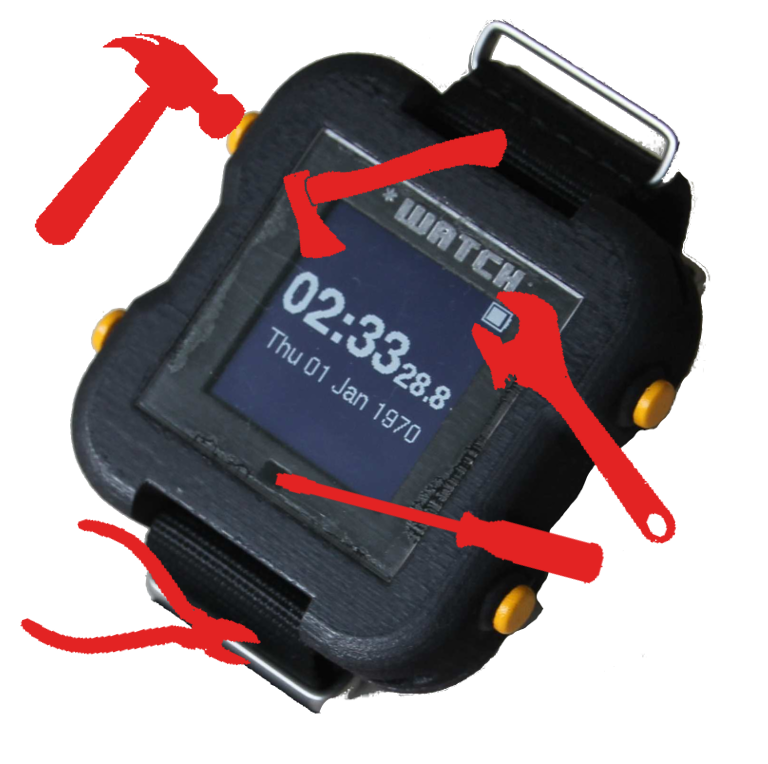
\includegraphics[height=7.5cm]{fwatch-full-side-tool.eps}
    }{
      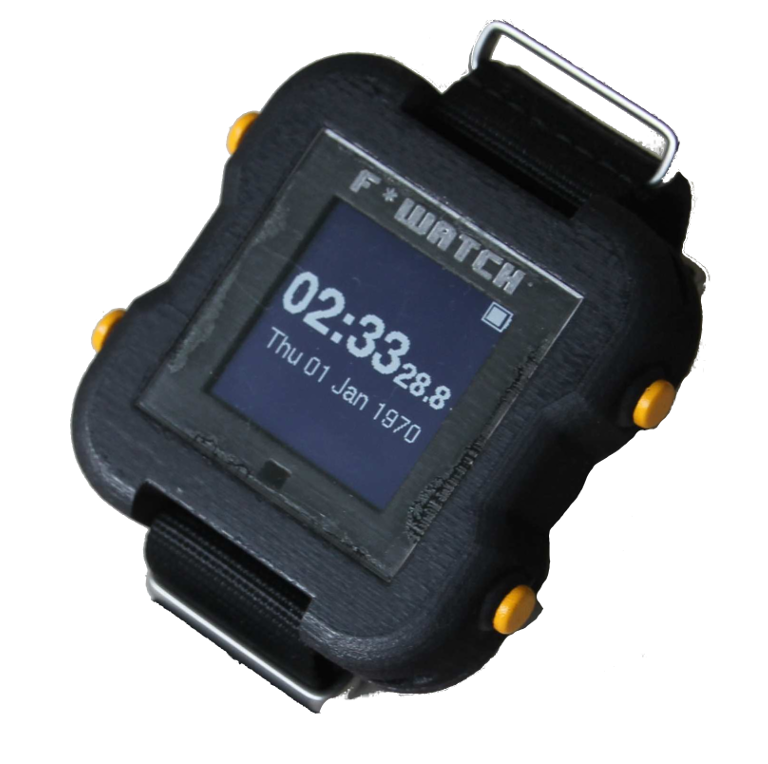
\includegraphics[height=7.5cm]{fwatch-full-side.eps}
    }
  \end{center}

  \note[item]{Software is really easy to share}
  \note[item]{Hardware sharing depends on tool and file format ---}

  \note[item]{The first consideration. For a free development we
    absolutely need free file format and tools to ease sharing}
  \note[item]{.doc MS office example}
  \note[item]{it was a pain}
  \note[item]{today, comparable}
  \note[item]{CERN experience}
\end{frame}

%------------ FRAME --------------------------------------------------

\begin{frame}{Easy to Made}
  \Large
  \begin{center}
    How difficult can be? \\
    \vskip 1cm
    Competitive free tools \\
    \vskip 1cm
    Specialized company in 3D printing \\
    \vskip 1cm
    Specialized company in PCB printing \\
    \vskip 1cm
    Easy to ship everywhere
 \end{center}

  \note[item]{The second consideration is that today is so easy the
    step from the idea to product}
\end{frame}

%------------ FRAME --------------------------------------------------

\begin{frame}{Next Generation Free-Open Source}
  \Large
  \begin{center}
    Free product are real \\
    \vskip 1cm
    cars, robots, watches, bikes, houses, phones, ... \\
    \vskip 1cm
    3D Metal printers \\
  \end{center}

  \note{Just talk a bit about it}
\end{frame}

%------------ FRAME --------------------------------------------------

\begin{frame}{Please Join}
  \Large
  \begin{center}
    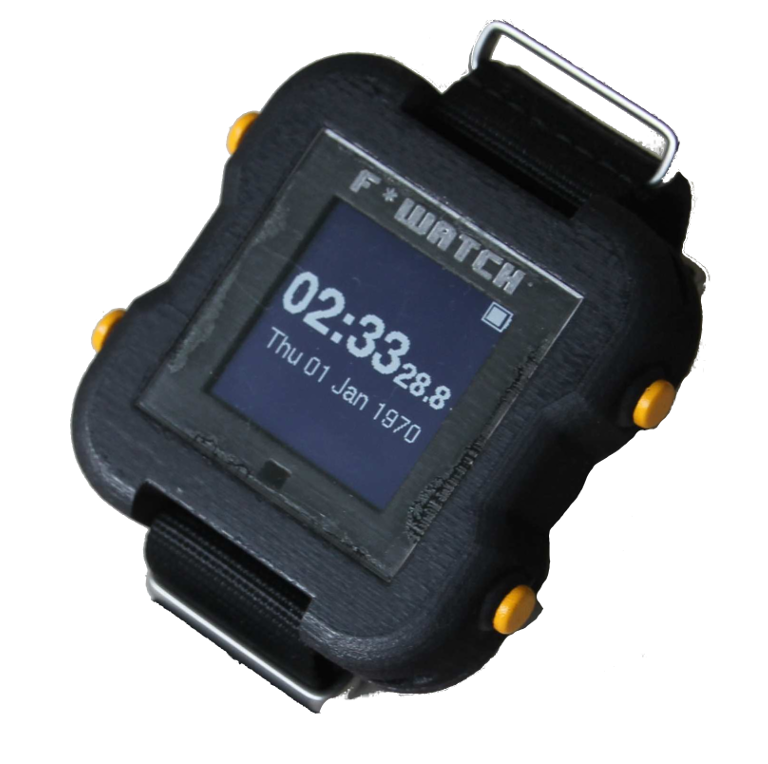
\includegraphics[height=3.5cm]{fwatch-full-side.eps} \\
    \vskip 5mm
    Far away from a real product \\
    \vskip 5mm
    Make it a good example \\
    \vskip 5mm
    Join the project \\
  \end{center}

  \note[item]{not a real product}
  \note[item]{it would be good to have a mechanical expert}
  \note[item]{company can do it better}
  \note[item]{in general join the project}
  \note[item]{make it a good example}
\end{frame}


\begin{comment}
\end{comment}


\end{document}


